%!TEX root = ../lectures_olympics.tex

\chapter{静磁场}
相信很多同学都玩过吸铁,了解一些基本的磁现象。
磁铁有南北两极,物理上南极用$S$表示,北极用$N$来表示,和电荷类似它们之间的作用力同性相斥、异性相吸。
电现象和磁现象的相似之处仅限于此,除此之外它们满足截然不同的规律。

很长时间以来人们都认为电和磁是两种不同的、没有内在关联的自然现象。
但在随后的科学发展过程中,人们从偶然现象出发发现电和磁并不是没有关系,由电荷的定向流动--电流--能够产生磁场,通过磁场的变化就能够产生对电荷的作用力,最终人们认识到电和磁并不是孤立的对象,而是同一种自然现象的两种不同表现形式而已。
在此基础上人们建立了{\heiti 电磁学}(elecromagnetism),极大地推动了人类技术的发展,造就了第二次工业革命,拿到了打开近代世界大门的钥匙。
在本章和随后的几章当中我们将从基本的磁现象出发逐渐深入到电磁现象的本质当中。


\section{电磁场中带电粒子的运动}

首先让我们回答一个问题:磁场是什么。最初人们通过小磁铁之间的相互作用感受磁场,奥斯特({\itshape H. C. \O rsted})的实验首次揭示出电流可以产生磁场而使磁体偏转。很自然地根据牛顿第三定理,磁体对电流的力实际上是磁体产生的磁场对电流的力。那么电流与电流之间也理应由于电流产生的磁场而产生相互作用。安培({\itshape A.-M. Amp\`ere})的实验有效地支持了这一点并总结出了磁场满足的基本规律。后来,人们又发现磁铁的磁性来源于磁铁内部的分子电流。而电流实际上就是运动的电荷。至此人们恍然大悟:原来运动的电荷会产生磁场,而所谓磁场描述的正是其对运动电荷的作用。

所以运动电荷在磁场中的受力定义了{\heiti 磁场}(magnetic field)的值---{\heiti 磁感应强度}(magnetic flux density),单位是特斯拉$\unit{Tesla}, \unit{T}$。
当一个电荷为$q$,速度为$\vec{v}$的粒子在磁场$\vec{B}$当中运动时,它将受到大小和方向为
\begin{equation}\label{eqn: mag-Lorentz-force}
\vec{F} = q \vec{v}\times \vec{B}
\end{equation}
的磁场力的作用,这个力称之为{\heiti 洛伦兹力}(Lorentz force)\footnote{电磁场其实是一个整体的场。这个场对以$\vec{v}$运动的电荷$q$的作用力为$\vec{F}=q(\vec{E}+\vec{v} \times \vec{B})$。这个力才是普遍意义下的洛伦兹力,它同时定义了电场与磁场矢量的值}。
从洛伦兹力的表达式能够看出,它是一个时刻垂直于速度和磁力线的力,所以在洛伦兹力永远不会对运动的带电粒子作功。

在匀强磁场中带电粒子的运动具有极其显著的特点。
当某一时刻电量为$q$,质量为$m$的带电粒子的速度与磁场方向垂直,根据洛伦兹力的表达式\ref{eqn: mag-Lorentz-force}可知,所受磁力与速度方向垂直,大小$F = qvB$。
因为受力方向与速度方向垂直,带电粒子速度方向将发生改变。
简单的分析可知此后粒子将做匀速圆周运动,其向心心完全由洛伦兹力提供:
\begin{equation}
qBv = m\frac{v^2}{R},
\end{equation}
从上式可解出其圆形轨迹的半径与已知物理量的关系:
\begin{equation}
R = \frac{mv}{qB} = \frac{p}{qB}.
\end{equation}
从中可以看出,粒子轨道半径正比于其动量,反比于带电量和磁感应强度的乘积。
进一步可知飞行的周期
\begin{equation}
T = \frac{2\pi R}{v} = \frac{2 \pi m}{qB}.
\end{equation}
一个有趣的事实是圆周运动的周期与其速度的大小无关,只依赖于带电粒子本身的性质。
在给定磁场大小为已知的情况下,运动周期正比于粒子的质量,反比于其电量,或者说周期依赖于粒子的{\heiti 荷质比$\gamma=q/m$}(charge-to-mass ratio),它是一个标志微观粒子性质重要的物理量。
其它情况下带电粒子在磁场中的运动也可根据洛伦兹力的大小和方向通过力学的方法得到。



%%%%%%%%%%%%%%%%%
\begin{example}

宇宙空间某区域有一磁感应强度大小为$B=1.0\pow{-9}\unit{T}$的均匀磁场,现有一电子绕磁力线做螺旋运动。
该电子绕磁力线旋转一圈所需的时间间隔为 \kong\kong s;
若该电子沿磁场方向的运动速度为$1.0\pow{-2}c$,$c$为真空中光速的大小,则它在沿磁场方向前进$1.0\pow{-3}$光年的过程中,绕磁力线转了\kong\kong 圈。
已知电子电荷量为$1.60\pow{-9}\unit{C}$,电子质量为$9.11\pow{-31}\unit{kg}$。

\tagged{student}{\vspace*{4cm}}
\begin{taggedblock}{teacher}
\noindent
解析:$3.6*10^-2,8.8*10^7$
\end{taggedblock}
\end{example}
%%%%%%%%%%%%%%%%%%%%%%



\begin{example}
一个质量为$m$、电荷为$q$的带电粒子以速度$v$射入匀强磁场$B$当中,忽略重力的影响,试定性讨论此后该粒子的运动。
\begin{flushright}
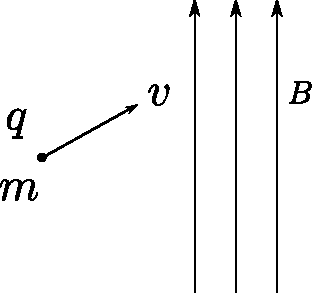
\includegraphics[width=0.3\textwidth]{images/mag-7.pdf} 
\end{flushright}
\tagged{student}{\vspace*{3cm}}
\begin{taggedblock}{teacher}
\noindent
解析:带电粒子的速度可以分解为平行和垂直于磁场方向的分量,$v_1$和$v_2$。
它只会受到洛伦兹力的作用,并且根据力的性质,它没有沿着磁场方向的分量,垂直于磁场和速度方向上的分量则是$qv_2B$,方向由速度向磁场的右手螺旋法则确定,需要注意的是带电粒子的电量的正负也会对力的方向产生影响。

平行于磁场方向不受力,所以速度大小不变。
垂直于磁场方向上受洛伦兹力作用下作圆周运动,设圆周运动的半径为$r$,它可由牛顿第二定律
\[qv_2B = \frac{mv_2^2}{r},\qquad r = \frac{mv_2}{qB}\]
给出。
所以在最一般的情况下粒子将做螺旋线运动,如果初速度方向和磁场方向垂直的话,则会做一个平面内的匀速圆周运动,其轨迹由初速度方向以及所受洛伦兹力方向决定。
\end{taggedblock}
\end{example}

%%%%%%%%%%%%%%%%%


\begin{example}

半径为$R$的圆柱形区域内有强度为$B$的匀强磁场,方向垂直于纸面向内。
在此区域的最低点$A$处有一个电子枪能向各个方向发射初速度为$v$的电子,通过调节电子初速度,使其在磁场中做圆周运动的半径也为$R$。
证明入射电子最终都沿水平方向射出磁场区域。
\tagged{student}{\vspace*{4cm}}
\begin{taggedblock}{teacher}
\newline
解析:找几何关系。四条边都相等的四边形为菱形。
\end{taggedblock}
\end{example}
%%%%%%%%%%%%%%%%%%%%%%

%%%%%%%%%%%%%%%%%%%%%%%%%%%%%%%%%%
\begin{example}
在真空中建立一坐标系,以水平向右为$x$轴正方向,竖直向下为$y$轴正方向,$z$轴垂直于纸面向里。
在$o\le y\le L$的区域内有匀强磁场,$L= 0.8\unit{m}$,磁场的磁感应强度方向沿$z$轴正方向,其大小$B = 0.10\unit{T}$。
今把一个荷质比$q/m = 50\unit{C\cdot kg^{-1}}$的带正电质点在$x=0,y=-0.2\unit{m},z = 0$处静止释放,将带电质点过原点的时刻定为$t=0$,求带电质点在磁场中任一时刻$t$的位置坐标。
并求它刚离开磁场时的位置和速度,简单起见取重力加速度$g = 10\unit{m/s^2}$。
\begin{flushright}
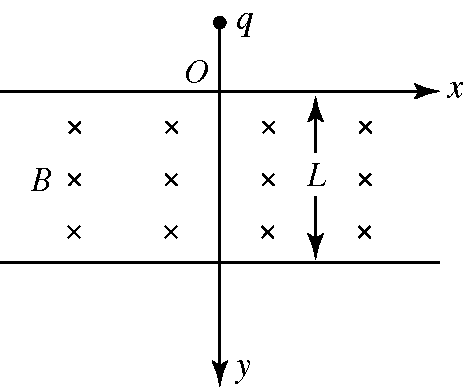
\includegraphics[width=0.4\textwidth]{images/mag-27.pdf}
\end{flushright}
\tagged{student}{\vspace*{4cm}}
\begin{taggedblock}{teacher}
\noindent
解析:算出:$v_0=2m/s,R=0.56m,\omega=5rad/s,\alpha=\frac{\pi}{4},x_O'=0.4,y_O'=0.4$\[x=v_0t-[R\sin(\omega t+\alpha)-x_0']\]
\[y=y_O'-R\cos(\omega t+\alpha)\]
刚离开磁场时:$v_x=4m/s,v_y=2m/s,y=-0.8m,x=0.63m$
\end{taggedblock}
\end{example}


%%%%%%%%%%%%%%%%%%%%%%%%%%






%%%%%%%%%%%%%%%%%
\begin{example}
在三维直角坐标中,沿$+z $方向有磁感强度为$B $的匀强磁场,沿$−z$ 方向有电场强度为$E$的匀强电场。
在原点$O $有一质量为$m $、电量为$−q $的粒子(不计重力)以正$x$方向、大小为$v$的初速度发射。
试求粒子再过$z $轴的坐标与时间。
\begin{flushright}
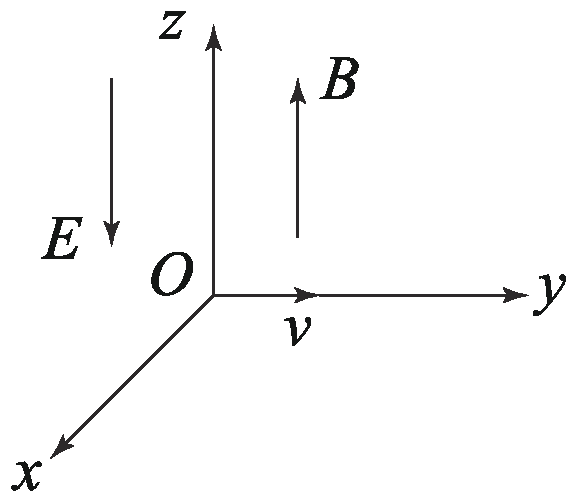
\includegraphics[width = 0.3\textwidth]{images/mag-12.pdf} 
\end{flushright}

\tagged{student}{\vspace*{2cm}}
\begin{taggedblock}{teacher}
\noindent
解析:通过受力分析可知,带电粒子将在$x-y$平面上做匀速圆周运动,周期为$T = \frac{2\pi m}{qB}$,在$z$方向上匀加速运动,加速度为$\frac{qE}{m}$,这样在经过$n$个周期以后会再次经过$z$轴。
简单的计算可得
\[
t_n = nT = n \frac{2\pi m }{qB},\qquad z_n = \frac{1}{2}at_n^2 = \frac{2\pi^2mE}{qB^2}n^2,\qquad n=1,2,3\cdots
\]
\end{taggedblock}
\end{example}
%%%%%%%%%%%%%%%%%%%%%%


\begin{example}
如图所示的空间当中有正交的匀强电场$E$和匀强磁场$B$,其方向在图中标出。
一个质量为$m$的带电$q$的粒子从该电磁场区域的左侧进入,当它的速度取特定值时它能够沿直线通过该电磁场区域,求该特定的能量值$v$。
\begin{flushright}
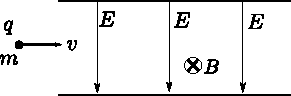
\includegraphics[width=0.3\textwidth]{images/mag-8.pdf} 
\end{flushright}
\tagged{student}{\vspace*{2cm}}
\begin{taggedblock}{teacher}
\noindent
解析:当带电粒子速度为$v$时,它将会受到$qE$的电场力和$qvB$的磁场力。
很明显,当两个力相等时它将没有竖直方向的分力,所以会沿直线通过。
从该式当中可以解出速度与电场、磁场大小的关系:
\[v = \frac{E}{B}\]
\end{taggedblock}
\end{example}



%%%%%%%%%%%%%%%%%
\begin{example}

在空间有相互垂直的匀强电场$E $和匀强磁$B$,电场方向为 $y$,磁场方向为$x$,一电子从原点$O $静止释放,求电子在$y$ 方向前进的最大距离。
\begin{flushright}
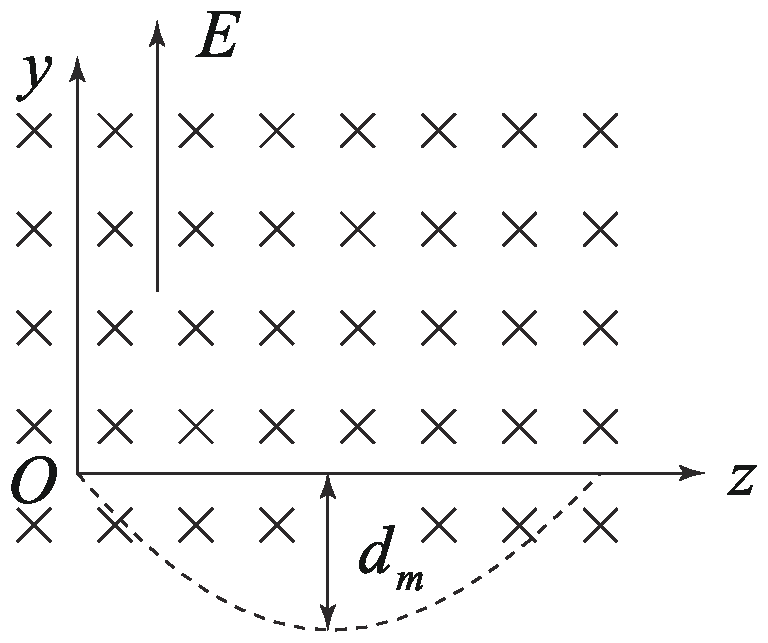
\includegraphics[width = 0.3\textwidth]{images/mag-13.pdf} 
\end{flushright}

\tagged{student}{\vspace*{4cm}}
\begin{taggedblock}{teacher}
\noindent
解析:设在y方向前进的最大距离为d,则此时电子只有沿x方向的速度分量。由能量守恒:\[Eed=\frac{1}{2}mv_x^2\]
由动量定理:\[m*\Delta v_x = F_x*\Delta t=Bev_y*\Delta t\]
求和得到:\[m*v_x=Bed\]
联立能量守恒方程得到:\[d=\frac{2mE}{B^2e}\]
\end{taggedblock}
\end{example}
%%%%%%%%%%%%%%%%%%%%%%




\newpage
\begin{example}
在图所示的装置中,离子源$A$可提供速度很小的正离子(其速度可视为0),经过加速电压加速后从$S$点进入匀强磁场,磁场方向垂直纸面指向纸外,虚线框为磁场区域的边界线。
在磁场作用下离子沿半个圆周运动后射出磁场,射出点$P$到$S$的距离用$x$表示。

1. 当离子源提供的是单一种类的第一种离子时,$P$到$S$的距离为$x_1$,当离子源提供的是单一种类的第二种离子时,$P$到$S$的距离为$x_2$,已知$\frac{x_1}{x_2} = \alpha$。
试求这两种离子在磁场中运动的时间$t_1$和$t_2$的比值$t_1/t_2$;

2. 若离子源$A$提供的是由$H^+$、$D^+$、$^4He^+$和$H_2^+$混合而成的多种离子,又通过速度选择器使各种离子的速率均为$v$,当这些离子从$S$点进入匀强磁场后,从磁场射出时可分离出哪几种离子束?
若$v = 2.0\pow{6}\unit{m/s}$,$B = 0.50\unit{T}$,基本电量$e = 1.60\pow{-19}\unit{C}$,质子质量$m_p = 1.68\pow{-27}\unit{kg}$,试求各种离子的射出点$P$到$S$的距离。
\begin{flushright}
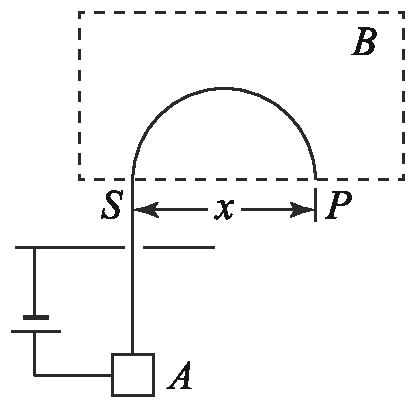
\includegraphics[width = 0.3\textwidth]{images/mag-30.pdf} 
\end{flushright}
\tagged{student}{\vspace*{4cm}}
\begin{taggedblock}{teacher}
\noindent
解析:$\frac{t_1}{t_2}=\alpha^2$
\\$x_{H^+}=8.4cm,x_{D^+}=17cm,x_{^4He^+}=34cm,x_{H_2^+}=17cm$
\end{taggedblock}
\end{example}


%%%%%%%%%%%%%%%%%
\begin{example}
从$z$轴上的$O$点发射一束电量为$q>0$、质量为$m$的带电粒子,它们速度方向分布在以$O$点为顶点、$z$轴为对称轴的一个顶角很小的锥体内(如图所示),速度的大小都等于$v$。
试设计一种匀强磁场,能使这束带电粒子会聚于$z$轴上的另一点$M$,$M$点离开$O$点的经离为$d$。
要求给出该磁场的方向、磁感应强度的大小和最小值。
不计粒子间的相互作用和重力的作用。
\begin{flushright}
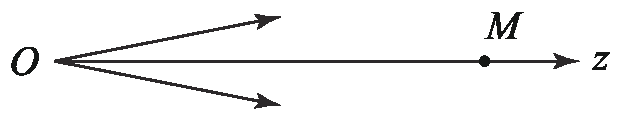
\includegraphics[width = 0.5\textwidth]{images/mag-31.pdf} 
\end{flushright}

\tagged{student}{\vspace*{4cm}}
\begin{taggedblock}{teacher}
\noindent
解析:沿$z$轴方向的匀强磁场,离子沿$z$方向可看成具有相同的速度,运动到$M$所需要的时间$t = \frac{d}{v}$,磁场的大小要求沿螺旋线运动的周期的整数倍刚好为这个时间:
\[
nT = n\frac{2\pi m}{qB} = t,\qquad B = \frac{2\pi mv}{qd}n.
\]
\end{taggedblock}
\end{example}
%%%%%%%%%%%%%%%%%%%%%%



%%%%%%%%%%%%%%%%%
\begin{example}
磁流体发电机的示意图如下,横截面积为矩形的管道长为$l$,宽为$a$,高为$b$,上下两个侧面是绝缘体,相距为$a$的两个侧面是电阻可忽略的导体,此两导体侧面与一负载电阻$R_L$相联,整个管道放在一匀强磁场中,磁感应强度的大小为$B$,方向垂直于上下侧面(向上)。
现在电离气体(正、负带电粒子)持续稳定流经管道,为了使问题简化,设横截面上各点流速相同。
已知流速与电离气体所受的摩擦阻力成正比;且无论有无磁场存在,都维持管两端电离气体压强差为$p$。
设无磁场存在时电离气体的流速为$v_0$,求有磁场存在时此磁流体发电机的电动势的大小$\mathcal{E}$。
已知电离气体的平均电阻率为$\rho$。
\begin{flushright}
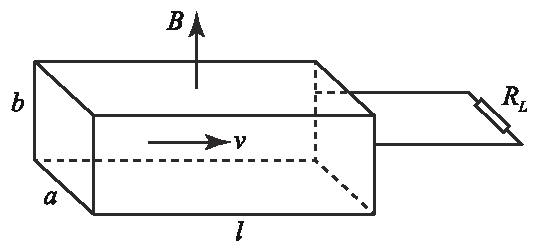
\includegraphics[width = 0.4\textwidth]{images/mag-37.pdf} 
\end{flushright}

\tagged{student}{\vspace*{3cm}}
\begin{taggedblock}{teacher}
\noindent
解析:$E=\frac{pBav_0(blR_L+pa)}{B^2alv_0+blR_LP+\rho ap}$
\end{taggedblock}
\end{example}
%%%%%%%%%%%%%%%%%%%%%%

\begin{example}
静止在匀强磁场中的放射性原子核$X$衰变为两个粒子$a$和$ b $,衰变后粒子 的运动速度与磁场垂直。
粒子$ a $ 和 $ b $的轨迹半径之比$ R_a:R_b = 45:1 $,周期之比$ T_a:T_b = 10:13 $,小圆被包含在大圆里。
已知该衰变过程中的释放的总能量$\Delta E$。
假定衰变过程中释放的核能全部转化成粒子的动能。求:

1. 粒子的电荷量之比$q_a/q_b$;

2. 粒子质量之比$m_a/m_b$;

3. 原子核$X$的电荷数和质量数$A$;

4. 粒子$a$的动能$E_a$。

\tagged{student}{\vspace*{4cm}}
\begin{taggedblock}{teacher}
\noindent
解析:1. 1:45
\\2. 2:117
\\3. 92号元素发生$\alpha $衰变,电荷数:92;质量数:238
\\4. $E_a=\frac{117}{119}\Delta E$
\end{taggedblock}
\end{example}

\newpage
\begin{example}
回旋加速器是利用磁场和电场共同使带电粒子作回旋运动,在运动中经高频电场反复加速的装置,它的主要结构是在磁极间的真空室内有两个半圆形的金属扁盒($D$形盒)隔开相对放置,$D$形盒上加交变电压,其间隙处产生交变电场。
置于中心的粒子源产生带电粒子射出来,受到电场加速,在$D$形盒内不受电场力,仅受磁极间磁场的洛伦兹力,在垂直磁场平面内作圆周运动。
假设磁场为匀强磁场,大小为$B$,求交变电压的周期。
假如$D$形盒的半径为$R$,求带电粒子出射的最大动能。
\begin{flushright}
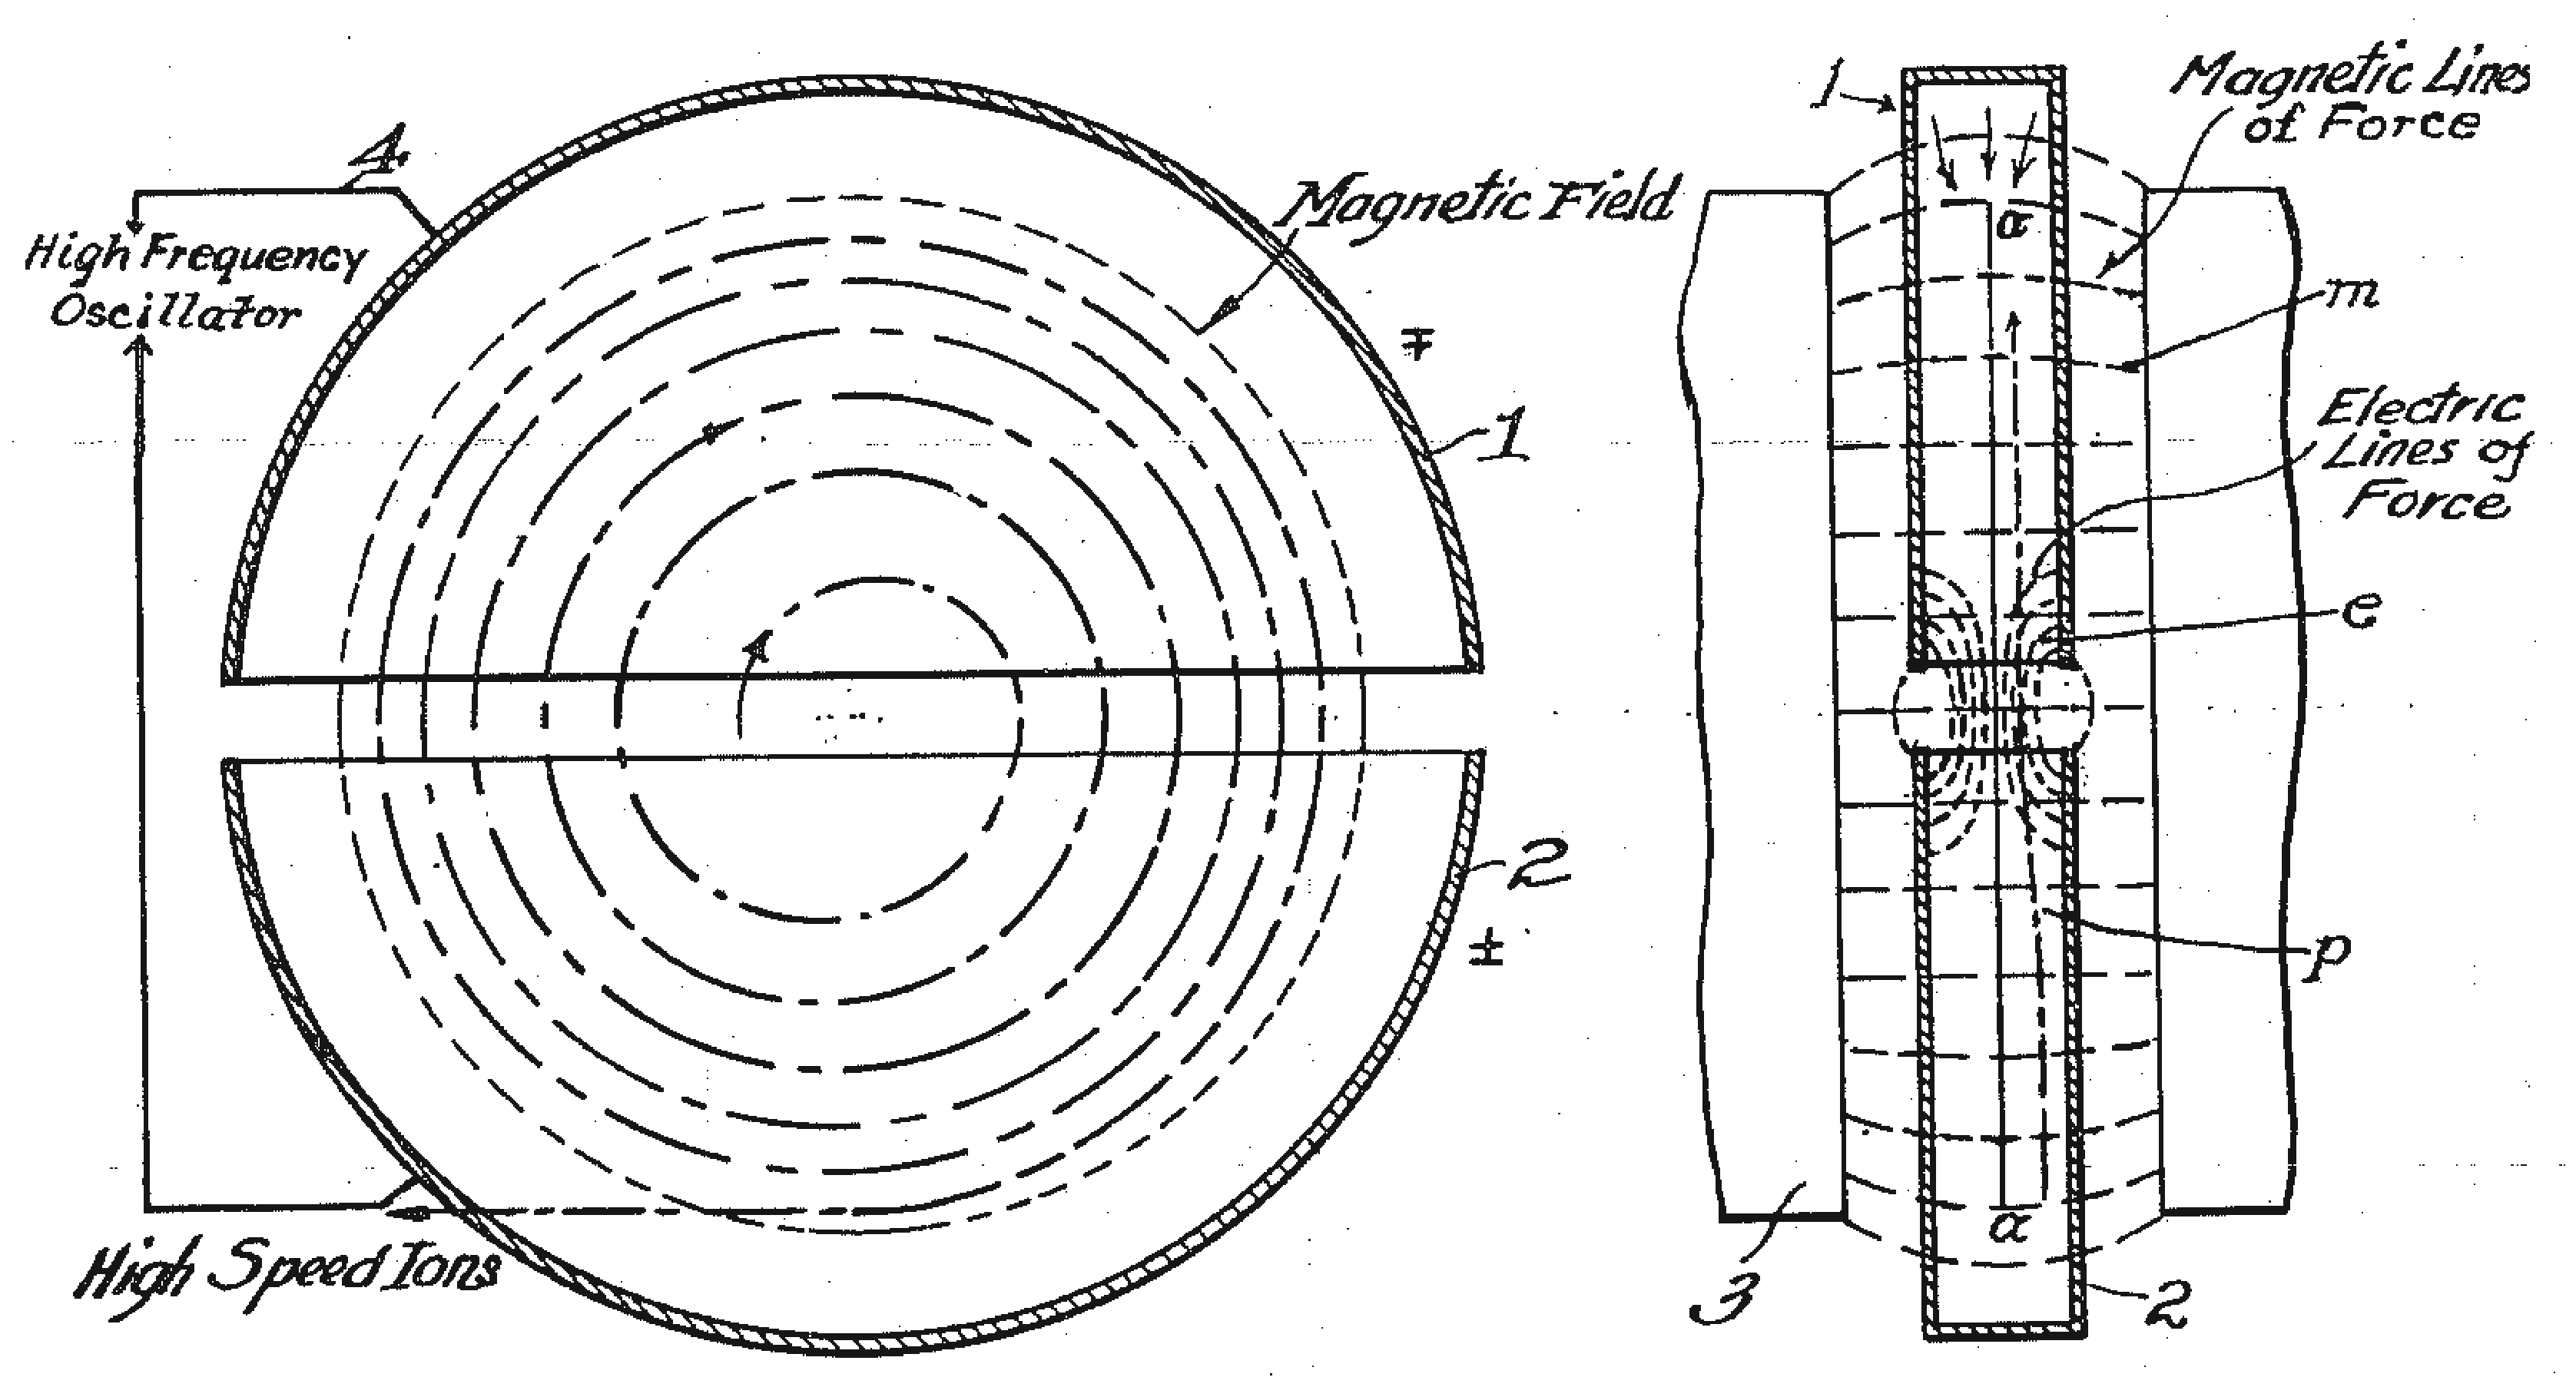
\includegraphics[width = 0.5\textwidth]{images/mag-38.pdf} 
\end{flushright}
\tagged{student}{\vspace*{2cm}}
\begin{taggedblock}{teacher}
\noindent
解析:1.周期:$\frac{\pi m}{Bq}$
\\2.动能:$\frac{B^2q^2R^2}{2m}$
\end{taggedblock}
\end{example}



\begin{example}
空间中有相互正交的匀强电场$E$和磁场$B$,求以任意初速度进入该电磁场区域内质量为$m$、电荷为$q$的带电粒子的轨迹。
\tagged{student}{\vspace*{4cm}}
\begin{taggedblock}{teacher}
\newline
解析:变换坐标系可知它的轨迹为匀速运动与匀速圆周运动的叠加。
如果有时间可以用微分方程求解。
\end{taggedblock}
\end{example}




\section{磁场中的电流}

简单起见,假设有一个匀强磁场,其大小用$B$来表示,在该匀强磁场当中有一段导线,其长度为$l$、电流为$I$并且与磁场方向垂直,此时磁场作用于该导线的力称做{\heiti 安培力}(Amp\`ere force),其大小方向与磁场、电流方向均垂直:
\begin{equation}
F=IBl
\end{equation}
方向由电流转向磁场方向的右手螺旋法则决定。

在最一般的情况下,静磁场的大小和方向有可能随空间位置的不同而变化,将磁场与空间位置的关系用函数$\vec{B}(\vec{r})$来表示,作用在整个导线上的安培力就是每段电流元所受到安培力
\begin{equation}
d\vec{F} = Id\vec{r}\times \vec{B}
\end{equation}
的矢量和:
\begin{equation}
\vec{F}=\oint Id\vec{r}\times \vec{B},
\end{equation}
其中的积分指对全部的电流回路的积分。


\begin{example}
试证明在匀强磁场当中无论电流回路取何种形状,它各个部分受到安培力的总和必为零。
\tagged{student}{\vspace*{4cm}}
\begin{taggedblock}{teacher}
\newline
解析:略
\end{taggedblock}
\end{example}

%%%%%%%%%%%%%%%%%
\begin{example}
试证明垂直于磁场静止放置的长度为$l$通有电流$I$的直导线所受的安培力为其中定向运动电子在磁场当中所受洛伦兹力的合力。
\tagged{student}{\vspace*{4cm}}
\begin{taggedblock}{teacher}
\newline
解析:设在匀强磁场$B$当中垂直于磁感线的导线内单位体积内的自由电子数为$n$,导线的截面积为$S$,电子平均速度为$v$,单个电子所受的洛伦兹力$f=evB$,方向垂直于导线。
这样所有电子的合力自然就是
\[F=nSl\cdot f = nSleBv = (neSv)Bl=IBl\]
可见洛伦兹力的合力就是安培力。
\end{taggedblock}
\end{example}



%%%%%%%%%%%%%%%%%
\begin{example}

质量分布均匀的细圆环,半径为$R $,总质量为$m$,让其均匀带正电,总电量为$q$,处在
垂直环面的磁感强度为$B$的匀强磁场中.令圆环绕着垂直环面并过圆心的轴转动,且角速度为$\omega$,转动方向和磁场方向如图所示。
求因环的旋转引起的环的张力的增加量。
\begin{flushright}
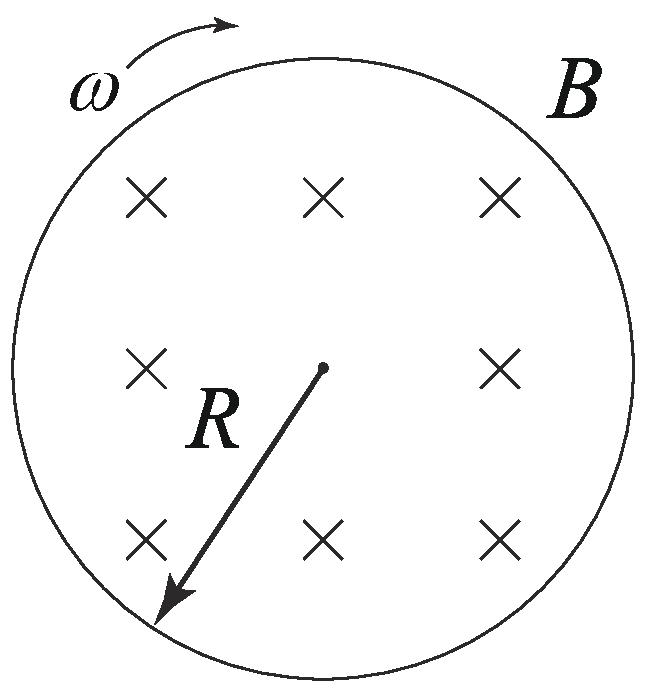
\includegraphics[width = 0.3\textwidth]{images/mag-11.pdf} 
\end{flushright}
\tagged{student}{\vspace*{2cm}}
\begin{taggedblock}{teacher}
\noindent
解析:$\Delta F=\frac{Bq\omega R}{2\pi}$
\end{taggedblock}
\end{example}
%%%%%%%%%%%%%%%%%%%%%%

\begin{example}
试证明如图所示在匀强磁场$B$当中的一个通有电流$I$的矩形回路所受到的合力为零,但合力矩不为零。
力矩的大小等于
\[\tau = Iab\cdot B\cdot \sin\theta\]
其中$a,b$分别为矩形线圈的两条边的边长,$\theta$为利用右手法则确定的回路垂线方向与磁场方向的夹角。
\begin{flushright}
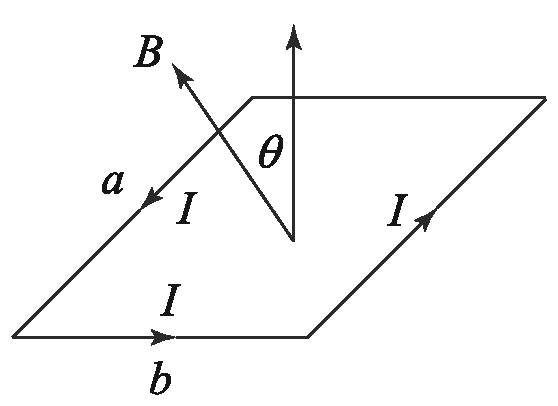
\includegraphics[width = 0.3\textwidth]{images/mag-9.pdf} 
\end{flushright}
\tagged{student}{\vspace*{2cm}}
\begin{taggedblock}{teacher}
\noindent
解析:略
\end{taggedblock}
\end{example}



%%%%%%%%%%%%%%%%%
\begin{example}
通电长导线中电流$I_0$的方向如图所示。
边长为$2L$的正方形载流线圈$abcd$中的电流强度为$I$,方向为$a\rightarrow b\rightarrow c\rightarrow d$。
线圈的$ab、cd $边以及过$ad、bc$边中点的轴线$OO'$都与长导线平行。
当线圈处于图示位置时,$ ab $边与直导线间的距离$aa_1$等于$2L$,且$aa_1$与$ad$垂直,已知长导线中电流产生的磁场在$ab $处的磁感应强度为$B_1$,在$cd$处的磁感应强度为$B_2$,则载流线圈处于此位置时受到的磁力矩(对$OO'$轴)的大小为\kong\kong。
\begin{flushright}
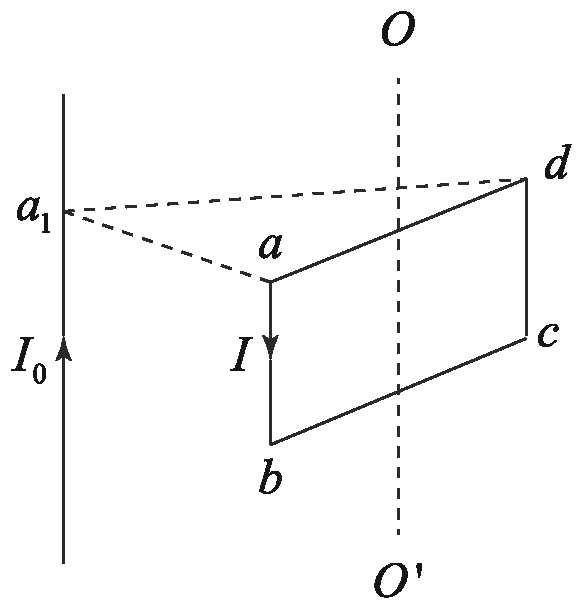
\includegraphics[width = 0.3\textwidth]{images/mag-10.pdf} 
\end{flushright}


\tagged{student}{\vspace*{2cm}}
\begin{taggedblock}{teacher}
\noindent
解析:ad、bc边所受的磁场力和转轴$OO'$平行,其力矩为零,ab、cd边受力大小分别为$F1=B_1I*2L$,$F2=B_2I*2L$,
\\F1、F2对转轴$OO'$的力臂分别为$L$和$\frac{\sqrt{2}}{2}L$,则两力对转轴的力矩为
\\$M=M_1+M_2=F_lL+F_2\frac{\sqrt{2}}{2}L=IL^2(2B_1+\sqrt{2}B_2)$
\end{taggedblock}
\end{example}
%%%%%%%%%%%%%%%%%%%%%%



%%%%%%%%%%%%%%%%%
\begin{example}
如图所示,两条平行的长直金属细导轨$KL、PQ$固定于同一水平面内,它们之间的距离为$l$,电阻可忽略不计;$ab$和$cd$是两根质量皆为$m$的金属细杆,杆与导轨垂直,且与导轨良好接触,并可沿导轨无摩擦地滑动。
两杆的电阻皆为$R$。
杆$cd$的中点系一轻绳,绳的另一端绕过轻的定滑轮悬挂一质量为$M$的物体,滑轮与转轴之间的摩擦不计,滑轮与杆$cd$之间的轻绳处于水平伸直状态并与导轨平行。
导轨和金属细杆都处于匀强磁场中,磁场方向垂直于导轨所在平面向上,磁感应强度的大小为$B$。
现两杆及悬物都从静止开始运动,当$ab$杆及$cd$杆的速度分别达到$v_1$和$v_2$时,两杆加速度的大小各为多少?
\begin{flushright}
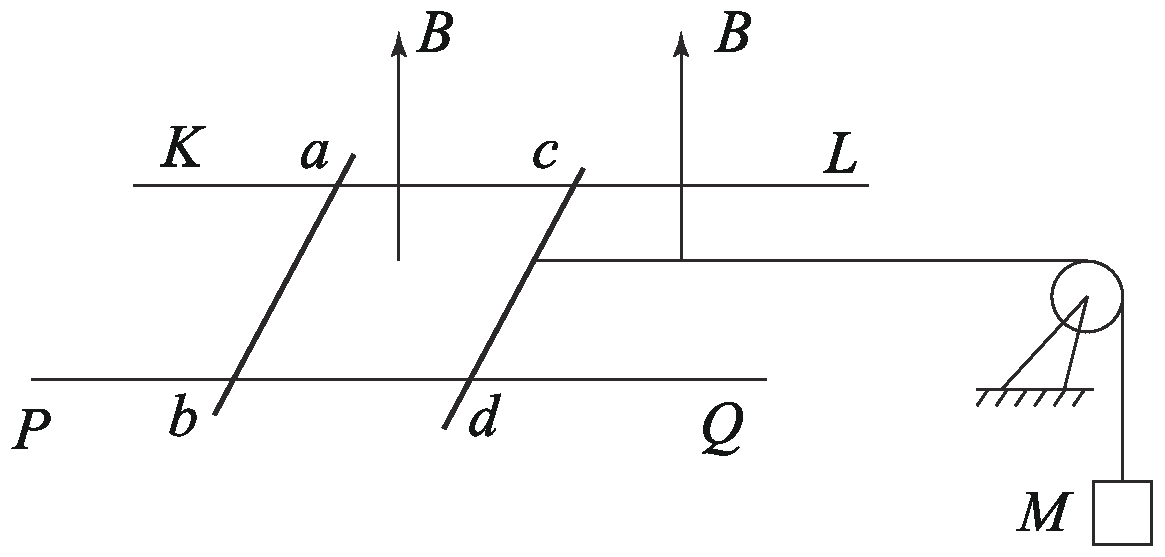
\includegraphics[width = 0.5\textwidth]{images/mag-21.pdf} 
\end{flushright}

\tagged{student}{\vspace*{4cm}}
\begin{taggedblock}{teacher}
\noindent
解析:ab与cd切割磁感线产生的感应电动势分别为:
\[E_1=Blv_1,E_2=Blv_2\]
总电动势\[E=E_2-E_1=Bl(v_2-v_1)\]
由闭合电路的欧姆定理可得,电路电流\[I=\frac{E}{R+R}=\frac{Bl(v_2-v_1)}{2R}\]
金属细杆受到的安培力大小\[F=BIl= \frac{B^2l^2(v_2-v_1}{2R}\]
设绳子对cd的拉力为T,由牛顿第二定律得:
ab棒:\[\frac{B^2l^2(v_2-v_1)}{2R}=ma_1\]
\[a_1= \frac{B^2l^2(v_2-v_1)}{2mR}\]
cd棒与M组成的系统:
\[Mg- \frac{B^2l^2(v_2-v_1)}{2R}=(M+m)a_2\]
由以上三式解得:\[a_2= 2MgR-\frac{B^2l^2(v_2-v_1)}{2(M+m)R}\]
答:当ab杆及cd杆的速度分别达到v1和v2时,两杆加速度的大小分别为:\[\frac{B^2l^2(v_2-v_1)}{2mR},\frac{2MgR-B^2l^2(v2-v1)}{2(M+m)R}\]
\end{taggedblock}
\end{example}
%%%%%%%%%%%%%%%%%%%%%%
对位于一个平面内的通电导线圈,即{\footnote 磁偶极子}(magnetic dipole)还有一个重要的物理量--{\heiti 磁矩}(magnetic moment)\footnote{注意根据国际电工委员会IEC的标准,磁矩需要与另一个概念--{\heiti 磁偶极矩}(magnetic dipole moment)区分开来。尽管后者十分像是前者的全称但可惜并不是,它等于前者乘以真空磁导率$\mu_0$}。
磁矩被定义为电流强度与导线所围的面积的乘积:
\begin{equation}
\mu = IS,
\end{equation}
同时它还是一个矢量,其方向由电流方向的右手螺旋法则确定。
当处于匀强磁场当中的通电导线所受到的力矩可以用磁矩和磁场强度的向量积给出:
\begin{equation}\label{eqn: mag-磁矩和力矩关系}
\vec{\tau} = \vec{\mu} \times \vec{B},
\end{equation}
在磁场中的能量则可表达为磁矩与磁感应强度的矢量内积:
\begin{equation}
E_p = -\vec{\mu}\cdot \vec{B}
\end{equation}
通过其定义可以看出当磁矩方向与磁场方向一致时,线圈将处于势能最低的状态。

\begin{example}
垂直于光滑的平面有一个匀强磁场,在该平面上放置着柔软的通电导线,它可以在安培力作用下在平面内任意运动,假设导线内的电流不受它的形状的影响,求两种情况下最终导线的形状。
\begin{flushright}
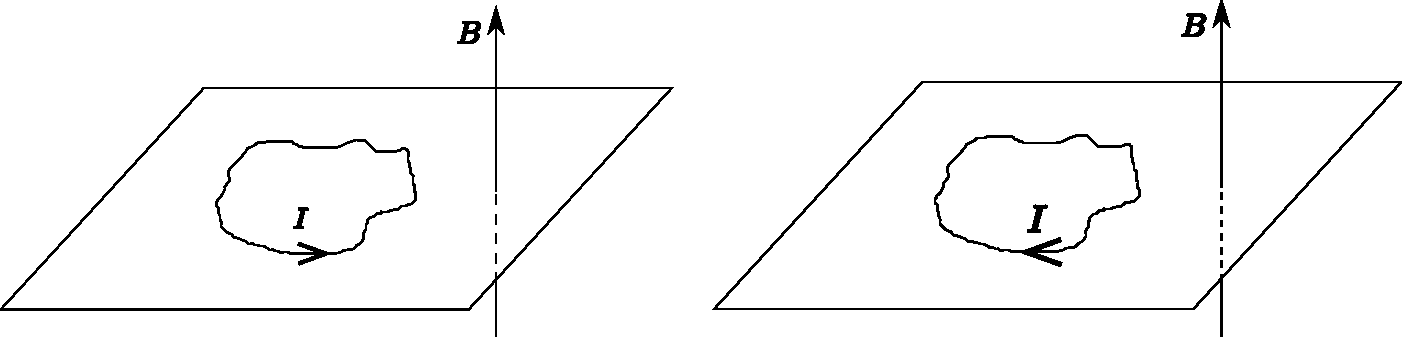
\includegraphics[width=0.5\textwidth]{images/mag-6.pdf} 
\end{flushright}
\tagged{student}{\vspace*{4cm}}
\begin{taggedblock}{teacher}
\noindent
解析:导线内部电流不会改变,但其形状会在安培力作用下自由地变化。
最终导线的形状一定是使总能量降为最低,对于第一种情况,当回路面积扩大时会有更大的磁矩,根据回路在磁场当中的能量可知它的能量会更小,所以最终导线将会变为圆形使其具有最大的面积。

第二种情况刚好相反,它的磁矩方向和磁场不一致,所以线圈面积越大能量则越高。
这样能量最低的状态反而是不断收缩以至于最后收成一点。

这个问题可进一步引申,当它并不是位于匀强磁场当中时,会受到平面方向的合力作用,无论哪种情况都是要跑到能量最低的可能状态。

\end{taggedblock}
\end{example}

\begin{example}
在经典物理学当中,当电量为$Q$、质量为$M$的均匀刚性带电的物体沿任意轴线做匀速转动时,它自转角动量与磁距的比值为一常数。
试给出该比值与所给物理量的关系。
\tagged{student}{\vspace*{4cm}}
\begin{taggedblock}{teacher}
\noindent
解析:从均匀带电和均匀质量分布的物体当中割出任意一小块,体积为$\delta V$,与轴线的距离为$r$,设旋转的角速度为$\omega$,它可看做是质量为$\delta m = \rho\delta V$,带电量为$\delta q = \rho_e\Delta V$的点电荷在距离为$r$处以角速度$\omega $转动。
它转动的等效电流
\[\delta I = \frac{\delta q}{T} = \frac{\rho_e \delta V }{2\pi/\omega} =\frac{\rho_e \omega}{2\pi}\delta V  \]
它对整体磁矩的贡献为
\[
\delta \mu = \delta I \cdot \pi r^2 = \frac{\rho_e  r^2}{2}\omega\delta V 
\]
同样的道理它转动起来的角动量为
\[
\delta L = \rho \delta V \cdot r^2\omega
\]
可以看到它们之间的比值:
\[
\frac{\delta \mu}{\delta L} = \frac{\rho_2}{2\rho_m} = \frac{Q}{2M}
\]
只与质量与电荷的比值有关,与转动轴的位置、角速度均无关。

\end{taggedblock}
\end{example}


\section{电流产生的磁场}
最后我们来研究电流产生的磁场。

上一章我们介绍了稳恒电流的概念。在稳恒电流中,除了形成电流的电荷是在不断地运动之外,体系的一切宏观参量都不会随时间改变。我们已经知道了导体中的电流需要由电场驱动,而电场本身是静电场,它由不变的电荷产生。现在我们还可以知道稳恒电流将产生不随时间改变的磁场,称为{\heiti 静磁场}(stactic magnetic field),研究静磁场的学问就叫{\heiti 静磁学}(magnetostatics)。
和电场类似地可以用{\heiti 磁感线}(magnetic field lines)来形象地表示一个磁场。
实验证明自然界找不到所谓的{\heiti 磁荷}(magnetic charge),所有的磁感线无一例外均是闭合的曲线\footnote{今后将会看到不但对于静止的磁场,随时间变化的磁场也满足这一性质}。

\begin{figure}[hbtp]
\centering
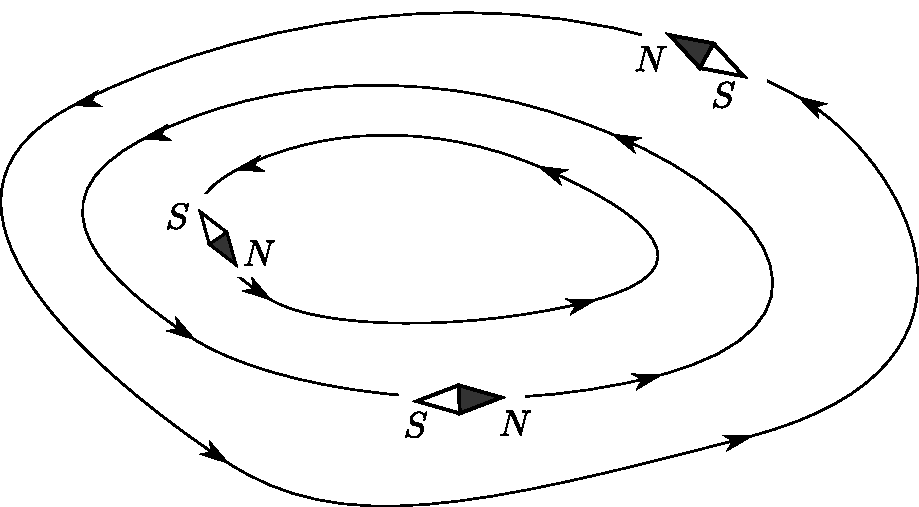
\includegraphics[width=0.5\textwidth]{images/mag-5.pdf}
\caption{磁感线的方向同静止在磁场中磁针方向的关系}
\end{figure}

在研究电场的性质时通过点电荷的电场出发,逐步推出复杂电荷分布下电场的性质。
与之有所不同的是,在磁场的研究过程当中我们却无法从“点电流”产生的磁场出发推出复杂电流产生磁场的性质,这是由于电荷守恒定律并不存在有一段孤立的电流,任何稳定的电流必然会形成一个回路。
尽管如此我们依然可以证明,任何一个电流回路产生的磁场等于将该回路无限分割以后形成的{\heiti 电流元}(current element)产生磁场的矢量和,每一段电流元可以看做一个矢量,它的大小正比于通过这一段导线的电流强度$I$与导线长度$dl$的乘积,方向则是由电流的方向所确定,从这个意义上讲电流元是一个空间当中的矢量。
如图\ref{fig: mag-biot-savart-law}所示的,每个电流元在空间当中给定点处产生的磁场正比于电流元的大小$Idl$,反比它们之间距离$r$的平方以及电流元方向与空间点与电流元之间的位置矢量夹角$\theta$的正弦;磁场的方向由电流元转向位置矢量$\vec{r}$的右手螺旋法则所决定:
\begin{equation}
d\vec{B} = \frac{\mu_0}{4\pi}\frac{Id\vec{l}\times \vec{r}}{r^3},
\end{equation}
其中$\mu_0/4\pi = 10^{-7}\unit{T \cdot m/A}$\footnote{注意在SI国际单位制的新提案中此等式将不再严格处理而是有一定误差,此提案预计将于2018年通过},$\mu_0$称为真空的磁导率,这就是描述电流产生磁场的{\heiti 毕奥-萨法尔定理}(Biot-Savart Law)。
完整的电流回路在给定点产生的磁场就是每段电流元产生磁场的矢量和:
\begin{equation}
\vec{B} =\frac{\mu_0}{4\pi} \oint \frac{Id\vec{l}\times \vec{r}}{r^3}
\end{equation}
\begin{figure}[hbtp]
\centering
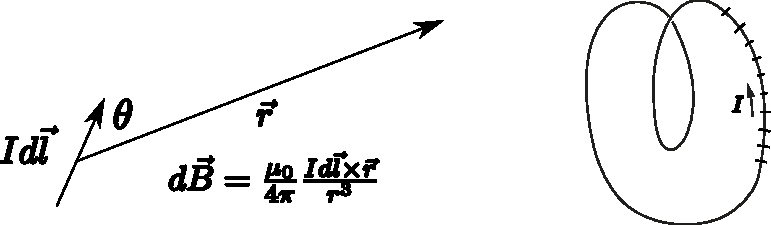
\includegraphics[width=0.7\textwidth]{images/biot-savart-law.pdf}
\caption{电流产生的磁场可以看成无限多个电流元产生磁场的叠加}\label{fig: mag-biot-savart-law}
\end{figure}


\subsection{安培环路定理}
利用毕奥-萨法尔定理计算电流的磁场的确是一件不容易的事情,就像在静电理论当中直接利用全空间的电荷分布来计算电场一样。
幸运的是除了利用毕奥-萨法尔定理静磁学当中我们还有一条类似于电场环路定理的用来决定电流产生磁场的定理称之为{\heiti 安培环路定理}(Amp\`ere's Circuital Law),它表明磁场沿着任意闭合回路的线积分正比于通过该回路的电流:
\begin{equation}
\oint \vec{B}\cdot d\vec{r} = \mu_0\sum I
\end{equation}
在电流分布有一定对称性时,通过安培环路定理可以得到磁场与电流的关系。

\subsection{磁高斯定理}

\begin{example}
通过安培环路定理证明通有电流$I$的无限长直导线在与它距离$r$处产生的磁感应强度大小为$B=\frac{\mu_0 I}{2\pi r}$。
\tagged{student}{\vspace*{4cm}}
\begin{taggedblock}{teacher}
\newline
解析:略
\end{taggedblock}
\end{example}


\begin{example}
通过安培环路定理证明通有电流$I$无限长螺线管内部为均匀磁场,其磁感应强度$B = \mu_0 nI$,其中$n$为单位长度内的匝数。
\tagged{student}{\vspace*{4cm}}
\begin{taggedblock}{teacher}
\newline
解析:略
\end{taggedblock}
\end{example}



%%%%%%%%%%%%%%%%%
\begin{example}

如图所示将均匀细导线做成的环上任意两点$A$和$B$与固定电源连接起来,计算由环上电流引起的环中心磁感应强度。
\begin{flushright}
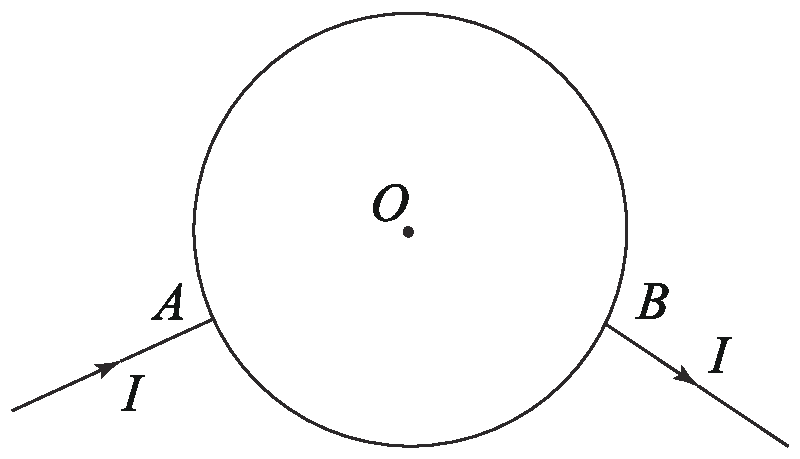
\includegraphics[width = 0.4\textwidth]{images/mag-36.pdf} 
\end{flushright}
\tagged{student}{\vspace*{2cm}}
\begin{taggedblock}{teacher}
\noindent
解析:0
\end{taggedblock}
\end{example}
%%%%%%%%%%%%%%%%%%%%%%






%%%%%%%%%%%%%%%%%%
%\begin{example}
%有一个长为$a$、宽为$b$的矩形导线框内通有电流$I$,它处于磁感应强度为$B$的匀强磁场,磁场和磁矩方向的夹角为$\theta$,利用各个导线所受安培力的大小证明此时导线框所受力矩满足式\ref{eqn: mag-磁矩和力矩关系}。
%\begin{flushright}
%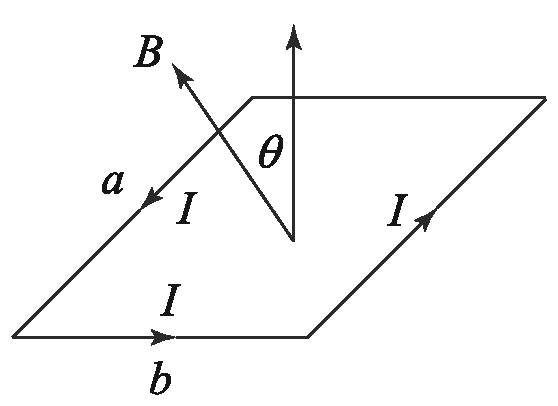
\includegraphics[width = 0.3\textwidth]{images/mag-9.pdf} 
%\end{flushright}
%
%\tagged{student}{\vspace*{2cm}}
%\begin{taggedblock}{teacher}
%\noindent
%解析:
%\end{taggedblock}
%\end{example}
%%%%%%%%%%%%%%%%%%%%%%%




